\documentclass[12pt]{article}

\usepackage{amsfonts,amsmath,amssymb,amsthm,boxedminipage,color,url,fullpage}
\usepackage{enumitem}
\usepackage{stmaryrd}
\usepackage[numbers]{natbib} % \citet{foo} -> Foo et al. [5]
\usepackage[pdfstartview=FitH,colorlinks,linkcolor=blue,filecolor=blue,citecolor=blue,urlcolor=blue]{hyperref} % blue links
\usepackage[labelfont=bf]{caption}
\usepackage{aliascnt,cleveref}
\usepackage{graphicx}

\usepackage{scribe}


% Useful Macros

% Bold font letters for vectors
\newcommand{\h}{{\mathbf h}}
\newcommand{\x}{{\mathbf x}}
\newcommand{\y}{{\mathbf y}}
\newcommand{\z}{{\mathbf z}}
\newcommand{\uu}{{\mathbf u}}
\newcommand{\vv}{{\mathbf v}}
\newcommand{\rr}{{\mathbf r}}
\newcommand{\w}{{\mathbf w}}
\newcommand{\s}{{\mathbf s}}
\newcommand{\e}{{\mathbf e}}
\newcommand{\aaa}{{\mathbf a}}
\newcommand{\bb}{{\mathbf b}}
\newcommand{\cc}{{\mathbf c}}
\newcommand{\dd}{{\mathbf d}}
\newcommand{\oo}{{\mathbf o}}
\newcommand{\p}{{\mathbf p}}

\newcommand\red[1]{{\color{red}#1}}
\newcommand\blue[1]{{\color{blue}#1}}
\newcommand{\mat}[1]{\llbracket#1\rrbracket} % Matricization operator
\newcommand{\matflex}[1]{\left\llbracket#1\right\rrbracket}
\newcommand{\otimesg}{\otimes_g}
\newcommand{\tenp}{\otimes} % Tensor/Outer product
\newcommand{\kronp}{\odot} % Kronecker product
\newcommand{\kharp}{\circ} % Khatri-Rao product
\newcommand{\hadmp}{*} % Hadamard product
\newcommand{\vect}[1]{\text{vec}\!( #1 )}  % Vectorization operator
\newcommand{\vectflex}[1]{\text{vec}\!\left( #1 \right)} 
\newcommand{\inprod}[2]  {\left\langle{#1},{#2}\right\rangle} % Inner product
\newcommand{\inprodnoflex}[2]{\langle{#1},{#2}\rangle}
\newcommand{\norm}[1]{\left\| #1 \right\|}
\newcommand{\normnoflex}[1]{\| #1 \|}
\newcommand{\ceil}[1]{\left\lceil #1 \right\rceil}

\newcommand{\A}{{\mathcal A}}
\newcommand{\B}{{\mathcal B}}
\newcommand{\T}{{\mathcal T}}
\newcommand{\U}{{\mathcal U}}
\newcommand{\V}{{\mathcal V}}
\newcommand{\W}{{\mathcal W}}
\newcommand{\X}{{\mathcal X}}
\newcommand{\Y}{{\mathcal Y}}
\newcommand{\OO}{{\mathcal O}}
\renewcommand{\L}{\mathcal{L}}
\newcommand{\EE}{\mathop{\mathbb E}} % Expectation operator

\newcommand{\eg}{{\it e.g. }}
\newcommand{\ie}{{\it i.e. }}
\newcommand{\cf}{{\it cf. }}

\graphicspath{ {./figs/} }

\begin{document}
	
	\makeheader{Adi Album \& Tomer Epshtein}								% your name
	{April 19, 2021}												% lecture date
	{6}																		 % lecture number
	{Optimization 1}			% lecture title
	
	\noindent
	In the course introduction we stated the Three Pillars of Statistical Learning: expressiveness, optimization and generalization.
	We completed the study of the first chapter - expressiveness.
	We shall now study optimization, \ie the procedure of updating model's weights in the attempt of minimizing loss on training data.
	
	
	\section{Optimization in deep learning is non-convex}
	In classical ML optimization was quite trivial. The target loss function was convex and therefore optimization schemes are guaranteed to reach global minimum.
	On the other hand, in DL, any reasonable training program is non-convex.
	We will prove non-convexity for a general case of settings. Consider a feed-forward fully connected NN with depth $N\geq2$ and activation $\sigma(\cdot)$:
	\begin{align} \label{eq:feed-forward fully connected NN}
		H = \{x \mapsto y = W_N(\sigma( W_{N-1}\sigma(W_{N-2}\sigma(\cdots W_2\sigma(W_1x))\cdots) | W_n\in\mathbb{R}^{d_n,d_{n-1}}, n\in [N]\} \}
	\end{align}
	
	\begin{proposition}
	\label{proposition:optimization in deep learning is non-convex}				
		Let $L(W_1,W_2,...,W_N)$ be a loss function that depends on $W_1,W_2,...,W_N$ only through the input-output mapping of the network.
		Assume that the global minimum of $L(\cdot)$ is attained for $W_1^\ast, W_2^\ast,...,W_N^\ast$.
		Assume also that this global minimum is smaller than the loss attainable with network having hidden widths $d_1=d_2=...=d_{N-1}=1$.
		Then $L(\cdot)$ is non-convex.
	\end{proposition}
	\begin{proof}
		Since $L(\cdot)$ depends on $W_1,W_2,...,W_N$ only through the input-output mapping, we may permute the rows of $W_1^\ast$, and correspondingly permute the columns of $W_2^\ast$, such that the value of $L(\cdot)$ is unchanged (still optimal).
		That is, for any permutation matrix
		$P\in\mathbb{R}^{d_1,d_1}$: $L(PW_1^\ast,W_2^{\ast}P^T,W_3^\ast,...,W_N^\ast)=L(W_1^\ast,W_2^\ast,...,W_N^\ast)=L^\ast$ (optimal loss value).
		\\Assume by contradiction that $L(\cdot)$ is convex. Then:
		\begin{align*}
    		L(\frac{1}{d_1!}\textstyle \sum_{P\ perm\ mat}{PW_1^\ast}, \frac{1}{d_1!}\textstyle \sum_{P\ perm\ mat} W_2^{\ast}P^T, W_3^\ast, ..., W_N^\ast) \leq
    		\\\frac{1}{d_1!}\sum_{P\ perm\ mat}L(PW_1^\ast,W_2^{\ast}P^T,W_3^\ast,...,W_N^\ast)=L^\ast
	    \end{align*}
	    Where $Q:=\frac{1}{d_1!}\sum_{P\ perm\ mat}P = \frac{1}{d_1}
	    \begin{bmatrix}
	        1 & \cdots & 1 \\
	        \vdots & \ddots & \vdots \\
	        1 & \cdots & 1
	    \end{bmatrix}$.
	    We Thus have an optimal weight setting where all the rows of $W_1$ are the same.
	    \\Continuing in this fashion, we can obtain an optimal weight setting $W_1,W_2,...,W_{N-1}$ whom each have their rows identical (\ie we may write $W_n=\vec{1}\overrightarrow{v_n}^T$ for $n\in[N]$ where $\vec{1}$ is the all-ones vector and $\overrightarrow{v_n}\in\mathbb{R}^{d_{n-1}}$. This contradicts the assumption of $L^\ast$ being smaller than loss attainable by network with hidden widths $d_1=d_2=...=d_{N-1}=1$. Thus $L(\cdot)$ is non-convex.
	\end{proof}
	\noindent\underline{Note:}
	\begin{itemize}
      \item The proposition (\ref{proposition:optimization in deep learning is non-convex}) and proof above can easily be extended to the case in which the NN includes biases.
      \item The result holds for any activation $\sigma(\cdot)$, including linear!
    \end{itemize}
	\begin{proposition}
	\label{proposition:optimization in deep learning is non-convex, other assumptions}				
		Let $L(W_1,W_2,...,W_N)$ be a continuously differentiable loss function that depends on $W_1,W_2,...,W_N$ only through the input-output mapping of the network.
		Assume that the global minimum of $L(\cdot)$ is not attained for $W_1=0,W_2=0,...,W_N=0$.
		Assume also that $\sigma(\cdot)$ is continuously differentiable and $\sigma(0)=0$.
		Then, $L(\cdot)$ is non-convex.
	\end{proposition}
	\begin{proof}
	    Homework...
	\end{proof}
	\section{Landscape approach}
	The landscape approach is built on the premise that if a non-convex objective has no bad local minima and no non-strict saddles, running GD (or SGD) over it will yield global minimum. Such results are typically established using two principles:
	\begin{itemize}
      \item GD reaches stationary (critical) points
      \item GD escapes strict saddles
    \end{itemize}
    \subsection{Convergence to stationary point}
    We will show that on any smooth objective, GD with sufficiently small step size converges to (approximate) stationary point in polynomial time.
	\begin{definition}
	\label{def:beta smooth function}				
		A differentiable function $f:\mathbb{R}^d\to\mathbb{R}$ is \underline{$\beta$-smooth} if its gradient is $\beta$-Lipschitz, \ie:
		\begin{align*}
		    \forall\overrightarrow{w_1},\overrightarrow{w_2}\in\mathbb{R}^d:\norm{\nabla{f(\overrightarrow{w_1})}-\nabla{f(\overrightarrow{w_2})}}\leq \beta \norm{\overrightarrow{w_1}-\overrightarrow{w_2}}
	    \end{align*}
	\end{definition}
	\begin{lemma}
	\label{lem:twice continuously differentiable beta-smooth functions property 1}
		Let $f:\mathbb{R}^d\to\mathbb{R}$ be twice continuously differentiable and $\beta$-smooth. Denote by $\nabla^2f(\overrightarrow{w})[\cdot,\cdot]$ the bilinear symmetric operator corresponding to the Hessian of $f(\cdot)$ at $\overrightarrow{w}$. Then, for any $\overrightarrow{v}\in\mathbb{R}^d$ it holds that $|\nabla^2f(\overrightarrow{w})[\overrightarrow{v},\overrightarrow{v}]|\leq\beta\cdot\norm{\overrightarrow{v}}^2$.
	\end{lemma}
	\begin{proof}
	    Define $h:\mathbb{R}\to\mathbb{R}$ by $h(t)=\langle\overrightarrow{v},\nabla{f(\overrightarrow{w}+t\overrightarrow{v})}-\nabla{f(\overrightarrow{w}})\rangle$.
	    \\From the chain rule we have:
		\begin{align*}
		    h'(0) = \nabla^2f(\overrightarrow{w})[\overrightarrow{v},\overrightarrow{v}]
	    \end{align*}
	    On the other hand, by $\beta$-smoothness of $f(\cdot)$:
		\begin{align*}
		    & \forall t\in\mathbb{R}: |h(t)| \leq \norm{\overrightarrow{v}}\cdot\norm{\nabla{f(\overrightarrow{w}+t\overrightarrow{v})}-\nabla{f(\overrightarrow{w}})} \leq \norm{\overrightarrow{v}} \cdot \beta \cdot \norm{\overrightarrow{w}+t\overrightarrow{v} - \overrightarrow{w}} = \beta \cdot t \cdot \norm{v}^2\\
		    & \Longrightarrow |h'(0)| \leq \beta \norm{\overrightarrow{v}}^2
	    \end{align*}
	    and the desired result follows.
	\end{proof}
	\begin{lemma}
	\label{lem:twice continuously differentiable beta-smooth functions property 2}
		Let $f:\mathbb{R}^d\to\mathbb{R}$ be twice continuously differentiable and $\beta$-smooth. Then:
		\begin{align*}
		    & \forall \overrightarrow{w_1}, \overrightarrow{w_2} \in \mathbb{R}^d :  |f(\overrightarrow{w_2}) - \underbrace{(f(\overrightarrow{w_1}) + \langle\nabla{f(\overrightarrow{w_1})}, \overrightarrow{w_2}-\overrightarrow{w_1}\rangle)}_\text{1\textsuperscript{st} order approx around $\overrightarrow{w_1}$}| \leq \frac{\beta}{2}\norm{\overrightarrow{w_2}-\overrightarrow{w_1}}^2
	    \end{align*}
	\end{lemma}
	\begin{proof}
	    Define $g:\mathbb{R}\to\mathbb{R}$ by $g(t)=f(\overrightarrow{w_1} + t(\overrightarrow{w_2}-\overrightarrow{w_1}))$. By Taylor's theorem:
		\begin{align*}
		    g(1) = g(0) + g'(0)\cdot(1-0) + \frac{1}{2}g''(\xi)\cdot(1-0)^2 \text{, for some $\xi\in(0,1)$}
        \end{align*}
	    Plugging in the definition of $g(\cdot)$ and employing the chain rule we get:
		\begin{align*}
		    f(\overrightarrow{w_2}) = f(\overrightarrow{w_1}) + \langle\nabla{f(\overrightarrow{w_1})},\overrightarrow{w_2}-\overrightarrow{w_1}\rangle + \frac{1}{2}\nabla^2{f(\overrightarrow{w_1}\cdot(1-\xi) + \overrightarrow{w_2}\cdot\xi)[\overrightarrow{w_2}-\overrightarrow{w_1},\overrightarrow{w_2}-\overrightarrow{w_1}]}
        \end{align*}
        The previous lemma (\ref{lem:twice continuously differentiable beta-smooth functions property 1}) implies that:
		\begin{align*}
		    |\nabla^2{f(\overrightarrow{w_1}\cdot(1-\xi) + \overrightarrow{w_2}\cdot\xi)[\overrightarrow{w_2}-\overrightarrow{w_1},\overrightarrow{w_2}-\overrightarrow{w_1}]}| \leq \beta\cdot\norm{\overrightarrow{w_2}-\overrightarrow{w_1}}^2
        \end{align*}
        Using this with the equality above yields the sought after result.
	\end{proof}
	\begin{definition}
	For a differentiable function $f:\mathbb{R}^d\to\mathbb{R}$ and $\epsilon\geq0$, we say that $\overrightarrow{w}\in\mathbb{R}^d$ is an \underline{$\epsilon$-stationary point} if $\norm{\nabla{f(\overrightarrow{w})}}\leq\epsilon$
	\\\underline{Note:} The usual term "Stationary Point" corresponds to the case $\epsilon=0$
	\end{definition}
	\begin{theorem}
	    \label{thm:convergence to epsilon stationary point}
	    \cite{1998-notes} \\
		Let $f:\mathbb{R}^d\to\mathbb{R}$ be a twice continuously differentiable and $\beta$-smooth function that attains its global minimum: $f^\ast = \min_{\overrightarrow{w}\in\mathbb{R}^d}{f(\overrightarrow{w})}$. Suppose we run GD over $f(\cdot)$ with step-size $\eta\leq\frac{1}{\beta}$ starting from $\overrightarrow{w_0}$. Then, for any $\epsilon>0$, an $\epsilon$-stationary point will be reached within a number of steps at most:
		\begin{align*}
		    \frac{2(f(\overrightarrow{w_0})-f^\ast)}{\eta\cdot\epsilon^2}
		\end{align*}
	\end{theorem}
	\begin{proof}
	    For every step $t\geq0$:
		\begin{align*}
		    f(\overrightarrow{w_{t+1}}) & \leq f(\overrightarrow{w_t}) + \langle\nabla{f(\overrightarrow{w_t})}, \overrightarrow{w_{t+1}} - \overrightarrow{w_t}\rangle + \frac{\beta}{2}\norm{\overrightarrow{w_{t+1}}-\overrightarrow{w_t}}^2 \\
		    & \leq f(\overrightarrow{w_t}) - \eta\norm{\nabla{f(\overrightarrow{w_t})}}^2 + \frac{\beta}{2}\eta^2\norm{\nabla{f(\overrightarrow{w_t})}}^2 \leq f(\overrightarrow{w_t}) - \frac{\eta}{2}\norm{\nabla{f(\overrightarrow{w_t})}}^2
		\end{align*}
		Assume that for steps $t=0,1,...,T-1: \norm{\nabla{f(\overrightarrow{w_T})}} > \epsilon$. Then:
		\begin{align*}
		    f(\overrightarrow{w_t}) < f(\overrightarrow{w_0}) - \frac{\eta}{2} \cdot T \cdot \epsilon^2
		\end{align*}
		Since by definition $f(\overrightarrow{w_T})\geq f^\ast$, we have:
		\begin{align*}
		    f^\ast < f(\overrightarrow{w_0}) - \frac{\eta}{2} \cdot T \cdot \epsilon^2 \Longrightarrow T < \frac{2(f(\overrightarrow{w_0}) - f^\ast)}{\eta \cdot \epsilon^2}
		\end{align*}
		Meaning the first step $t$ at which $\norm{\nabla{f(\overrightarrow{w_t})}}\leq\epsilon$ comes before step $\frac{2(f(\overrightarrow{w_0})-f^\ast)}{\eta \cdot \epsilon^2}$
	\end{proof}
	\subsection{Escaping strict saddle point}
	A \underline{strict saddle} is a stationary point that has at least one strictly negative eigenvalue to its Hessian (note that this definition can apply to a local maximum). We will consider a 2\textsuperscript{nd} order Taylor approximation around a strict saddle, and show that GD escapes it in reasonable time "with high probability".
	\\ Let $f:\mathbb{R}^d\to\mathbb{R}$ be a twice continuously differentiable function, with a strict saddle at $\overrightarrow{w_s}\in\mathbb{R}^d$. The 2\textsuperscript{nd} order Taylor approximation of $f(\cdot)$ around $\overrightarrow{w_s}$ is:
	\begin{align*}
	    \tilde{f}(\overrightarrow{w}) :&= f(\overrightarrow{w_s}) + \langle\nabla{f(\overrightarrow{w_s})}, \overrightarrow{w} - \overrightarrow{w_s}\rangle + \frac{1}{2}\nabla^2f(\overrightarrow{w_s})[\overrightarrow{w} - \overrightarrow{w_s}, \overrightarrow{w} - \overrightarrow{w_s}] \\
	    & = f(\overrightarrow{w_s}) + \frac{1}{2}\nabla^2f(\overrightarrow{w_s})[\overrightarrow{w} - \overrightarrow{w_s}, \overrightarrow{w} - \overrightarrow{w_s}] \\
	    & = f(\overrightarrow{w_s}) + \frac{1}{2}(\overrightarrow{w} - \overrightarrow{w_s})^T H (\overrightarrow{w} - \overrightarrow{w_s}) \\
	    & \text{(Where $H\in\mathbb{R}^{d,d}$ is a matrix representing bilinear operator $\nabla^2f(\overrightarrow{w_s})[\cdot,\cdot]$)}
	\end{align*}
	Its gradient: $\nabla{\tilde{f}(\overrightarrow{w})} = H(\overrightarrow{w} - \overrightarrow{w_s})$, yielding the following dynamics for GD:
	\begin{align*}
	    \overrightarrow{w_{t+1}} = \overrightarrow{w_t} - \eta \cdot H(\overrightarrow{w_t} - \overrightarrow{w_s})
	\end{align*}
	For $\epsilon>0$, we say that GD \underline{$\epsilon$-escaped} $\overrightarrow{w_s}$ if it reached a non-$\epsilon$-stationary point whose objective value is lower than that of $\overrightarrow{w_s}$, \ie if:
	\begin{enumerate}
      \item $\tilde{f}(\overrightarrow{w_t}) < \tilde{f}(\overrightarrow{w_s})$ ($=f(\overrightarrow{w_s}$))
      \item $\norm{\nabla{\tilde{f}(\overrightarrow{w_t})}} > \epsilon $
    \end{enumerate}
    Let $H = U \Lambda U^T$ be an orthogonal eigen decomposition for the (symmetric) matrix $H$,
    \\\ie\ $U\in\mathbb{R}^{d,d}$ is an orthogonal matrix ($UU^T=Id$) and $\Lambda\in\mathbb{R}^{d,d}$ is diagonal. Applying the change of variables $\overrightarrow{w} = U\overrightarrow{\theta} +\overrightarrow{w_s} \Longleftrightarrow \overrightarrow{\theta} = U^T(\overrightarrow{w} - \overrightarrow{w_s})$, we have:
	\begin{itemize}
      \item $\tilde{f}(\overrightarrow{w})$ - ${f}(\overrightarrow{w_s})$ = $\frac{1}{2}{\overrightarrow{\theta}}\Lambda{\overrightarrow{\theta}}^T$ = $\frac{1}{2}\sum_{i=1}^{d} \lambda_i{\theta_i}^{2}$  $(\Lambda=diag(\lambda_1, ..., \lambda_d))$
      \item $\left\lVert \nabla\tilde{f}(w) \right\lVert$ = $\left\lVert U\Lambda{\overrightarrow{\theta}} \right\lVert$ = $\left\lVert \Lambda{\overrightarrow{\theta}} \right\lVert$ = $({\sum_{i=1}^{d} {\lambda_i}^{2}{\theta_i}^{2}})^{0.5}$
      \item ${\overrightarrow{\theta}}^{(t+1)}$ = ${\overrightarrow{\theta}}^{(t)}$ - $\eta\Lambda{\overrightarrow{\theta}}^{(t)}$ $\Longleftrightarrow$ ${\theta_i}^{(t+1)}$ = $(1-\eta\lambda_i){\theta_i}^{(t)}$, $i \in[d]$
    \end{itemize}
    Establishing ${\epsilon}$-escaping thus means showing that under the dynamics of ${\theta_t}$ it holds that ${\sum_{i=1}^{d} {\lambda_i}{(\theta_i}^{(t)})^{2}} < 0 $ and ${\sum_{i=1}^{d} {\lambda_i}^{2}{(\theta_i}^{(t)})^{2}} > {\epsilon^{2}} $. Plugging in the dynamics, we may write these conditions as follows:
    
    \begin{enumerate}
      \item ${\sum_{i=1}^{d} {\lambda_i}{(1 - \eta\lambda_i)}^{2t}}{({\theta_i}^{(0)})}^{2} < 0 $
      \item ${\sum_{i=1}^{d} {{\lambda_i}^{2}}{(1 - \eta\lambda_i)}^{2t}}{({\theta_i}^{(0)})}^{2} > {{\epsilon}^{2}} $
    \end{enumerate}
    If the original objective $f(\cdot)$ is $\beta-smooth$, then by the lemma we've proven all eigenvalues of its Hessian are bounded in absolute value by $\beta$. This implies that $\norm {\lambda_i} \leq \beta , \forall {i \in [d]}$.
    Since $\overrightarrow{w_s}$ is a strict saddle, there exists some ${i \in [d]}$ for which ${\lambda_i} < 0 $. Assume W.L.O.G that ${\lambda_1} = -\alpha < 0 $. In the customary setting of step size $\eta \leq \frac{1}{\beta}$:
    
    ${\sum_{i=1}^{d} {\lambda_i}{(1 - \eta\lambda_i)}^{2t}{({\theta_i}^{(0)})}^{2}} \leq  $ $ {\lambda_1}{(1 - \eta\lambda_1)}^{2t}{({\theta_1}^{(0)})}^{2} + {\sum_{i\in[d]: {\lambda_i > 0}} {\lambda_i}{(1 - \eta\lambda_i)}^{2t}{({\theta_i}^{(0)})}^{2}}  $
    
    $ \leq {-\alpha}{(1 + \eta\alpha)}^{2t}{({\theta_1}^{(0)})}^{2} + {\sum_{i\in[d]: {\lambda_i > 0}} {\lambda_i}{({\theta_i}^{(0)})}^{2}} < 0 $ 
    
    Where we used ${{(1 - \eta\lambda_i)}^{2t} \in [0,1]}$  and require the last inequality $< 0$.
    
    $\Longleftrightarrow$
    
    ${(1 + \eta\alpha)}^{2t} > {\frac{\sum_{i\in[d]: {\lambda_i > 0}} {\lambda_i}{({\theta_i}^{(0)})}^{2}}{({\theta_1}^{(0)})^2\alpha}}$
    
    (Assuming ${\theta_1}^{(0)} \ne 0$)
    
    $\Longleftrightarrow$
    
    $t > \frac{\frac{1}{2}\log {\frac{\sum_{i\in[d]: {\lambda_i > 0}} {\lambda_i}{({\theta_i}^{(0)})}^{2}}{({\theta_1}^{(0)})^{2}\alpha}}}{\log {(1+\eta\alpha)}}$
    
	\newpage
	Additionally:
	\begin{align*}
	{\sum_{i=1}^{d} {{\lambda_i}^{2}}{(1 - \eta\lambda_i)}^{2t}{({\theta_i}^{(0)})}^{2}} \geq & {{\lambda_1}^{2}}{(1 - \eta\lambda_1)}^{2t}{({\theta_1}^{(0)})}^{2} \\
	& = {{\alpha}^{2}}{(1 + \eta\alpha)}^{2t}{({\theta_1}^{(0)})}^{2} > {{\epsilon} ^{2}}
	\end{align*}
	Where we require the last inequality $>\epsilon^{2}$
	\begin{align*}
	    \Longleftrightarrow
    	t > {\frac{1}{2}\log {({{\epsilon}^{2}} / { \alpha^2 ({\theta_1}^{(0)})^{2}})}} / {\log {(1+\eta\alpha)}} \\
    	\text{(Assuming ${\theta_1}^{(0)} \ne 0$)}
	\end{align*}
	Conditions 1 and 2 thus hold, \ie the saddle is $\epsilon$-escaped, after at most:
	\begin{align*}
	    \ceil{\frac{1}{2} \frac{log\left(\frac{max\{\sum_{i\in[d]: {\lambda_i > 0}} {\lambda_i (\theta_i^{(0)})}, \frac{\epsilon^2}{\alpha} \}}{{{\theta_1^{(0)}}^2}\alpha}\right)}{log(1+\eta\alpha)}} \text{ steps.}
	\end{align*}
	The reason we said efficient escaping occurs "w.h.p" is because of the dependence on $|{\theta_1}^{(0)}|$ - initial distance from $\overrightarrow{w_s}$ in the direction of negative curvature. The larger this is, the fastest the escape is guaranteed to be. If we initialize $\overrightarrow{w}$ ($\ie$  set $\overrightarrow{w_0}$) by an appropriately scaled isotropic random distribution centered at $\overrightarrow{w_s}$, we can assure that all the coordinates of $\overrightarrow{\theta_0}$ are w.h.p large "enough" (note that there is no need to know which directions have negative curvature).
	\subsection{Putting it all together}
	Combining the above principles - convergence to stationary point and escaping non-strict saddle point - into a formal result (guarantee of efficient convergence to stationary point with PSD Hessian) is a highly technical process, primarily since one needs to treat the discrepancy between ${2}^{nd}$ order Taylor approx and the original objective. We will not do this here. Instead, we will state an exemplar result, taken from \cite{avoid-saddle-point}.

    \begin{definition}
	\label{def:rho Hessian Lipschitz}				
		A twice differentiable function $f:\mathbb{R}^d\to\mathbb{R}$ is a  \underline{$\rho$-Hessian-Lipschitz} if:
		\begin{align*}
		    \forall\overrightarrow{w_1},\overrightarrow{w_2}\in\mathbb{R}^d:\norm{{{\nabla}^{2}}{f(\overrightarrow{w_1})}-{{\nabla}^{2}}{f(\overrightarrow{w_2})}}_{Spectral}
		    \leq
		    \rho\norm{\overrightarrow{w_1}-\overrightarrow{w_2}}
	    \end{align*}
	    For such function, we say that $\overrightarrow{w}$ is an \underline{$\epsilon-{{2}^{nd}}-order$ $stationary$ $point$} if:
	    \begin{align*}
		    \norm{{\nabla}{f(\overrightarrow{w})}} \leq \epsilon
	    \end{align*}
        \centerline{and}
	    \begin{align*}
            {\lambda_{min}}({{\nabla}^{2}}{f(\overrightarrow{w})}) 
		    \geq -\sqrt{\rho\epsilon}
	    \end{align*}
	\end{definition}
	\newpage
	\noindent\underline{Algorithm:}
	Perturbed Gradient Descent: PGD($\overrightarrow{w_0}, \beta, \rho, \epsilon, c, \delta, \Delta{f}):$
	\begin{enumerate}[label*=\arabic*.]
        \item $ x \leftarrow 3\max\{\log(\frac{d\beta \Delta f} {c \epsilon^2 \delta}),4\}$, $\eta \leftarrow \frac{c}{\beta}$, $r \leftarrow \frac{\sqrt{c}}{x^2}\cdot\frac{\epsilon}{\beta}$
        \item $ g_{thresh} \leftarrow \frac{\sqrt{c}}{x^2}\cdot\epsilon$, $ f_{thresh} \leftarrow \frac{c}{x^3}\cdot\sqrt{\frac{\epsilon^3}{\rho}}$, $t_{thresh} \leftarrow \frac{x}{c^2} \cdot \frac{\beta}{\sqrt{\rho\epsilon}}$
        \item $t_{noise} \leftarrow -t_{thresh}-1$
        \item for $t=0, 1, ..., d_0:$
        \begin{enumerate}[label*=\arabic*.]
            \item If $\norm{\nabla{f(\overrightarrow{w_t})}} \leq g_{thresh}$ and $t-t_{noise} > t_{thresh}$ then:
            \begin{enumerate}[label*=\arabic*.]
                \item $\overrightarrow{\tilde{w_t}} \leftarrow \overrightarrow{w_t}$, $t_{noise} \leftarrow t$
                \item {\label{uniform-sampling}}$\overrightarrow{w_t} \leftarrow \overrightarrow{\tilde{w_t}} + \overrightarrow{\xi_t}$, where $\overrightarrow{\xi_t} ~ $ is uniformly sampled over $\{\overrightarrow{w'}:\norm{\overrightarrow{w'}} \leq r\}$
            \end{enumerate}
            \item If $t-t_{noise} = t_{thresh}$ and $f(\overrightarrow{w_t}) - f(\overrightarrow{\tilde{w}_{t_{noise}}}) > -f_{thresh}$ then:
            \begin{enumerate}[label*=\arabic*.]
                \item return $\overrightarrow{\tilde{w}_{t_{noise}}}$
            \end{enumerate}
            \item $\overrightarrow{w_{t+1}} \leftarrow \overrightarrow{w_t} - \eta \cdot \nabla{f}(\overrightarrow{w_t})$
      \end{enumerate}
    \end{enumerate}
    \noindent\underline{Note}:
    Perturbation ${\xi_t}$ in \eqref{uniform-sampling} is needed in order to ensure sufficient distance from saddle in direction of negative curvature.
	\begin{theorem}
	\label{thm:PGD outputs epsilon-2nd-order-stationary point}
		Let $f:\mathbb{R}^d\to\mathbb{R}$ be a $\beta$-smooth and $\rho$-Hessian Lipschitz function with global minimum $f^\ast$. Then there exists an absolute constant $c_{max}$ s.t. for any $\delta>0$, $\epsilon \leq \frac{\beta^2}{\rho}$, $\Delta f \geq  f(\overrightarrow{w_0})-f^\ast$ and const $c \leq c_{max}$, PGD($\overrightarrow{w_0}, \beta, \rho, \epsilon, c, \delta, \Delta{f}$) will output an $\epsilon$-2\textsuperscript{nd}-order stationary point, w.p. $1-\delta$, and terminate in the following number of steps:
	    \begin{align*}
            \mathcal{O}\left(\frac{\beta(f(\overrightarrow{w_0})-f^\ast)}{\epsilon^2} \cdot \log^4({\frac{d \beta \Delta f}{\epsilon^2 \delta}})\right)
	    \end{align*}
	\end{theorem}
	\subsection{Example - linear neural networks}
	As a simple test-bed for the landscape approach, we will analyze \underline{linear neural networks} (LNN) - feed-forward fully connected NN with linear (no) activation. Note that in accordance with what wa've shown above, they induce non-convex training programs, even though their input-output mappings are linear.
	\newline
	A depth $N$ LNN with input dim $d_0 \in \mathbb{N}$, hidden dims $d_1, d_2, ..., d_{N-1} \in \mathbb{N}$, and output dim $d_N \in \mathbb{N}$, is the following parametric family of functions:
    \begin{align*}
        \{x \in \mathbb{R}^{d_0} \mapsto y = W_N W_{N-1} \cdots W_1 x \in \mathbb{R}^{d_N} : W_n \in \mathbb{R}^{d_n, d_{n-1}}, n\in [N]\}
    \end{align*}
    Given a LNN, for $1 \leq j \leq j' \leq N$ we denote: $W_{j:j'}:=W_{j'}W_{j'-1}\cdots W_j$. For convenience, if $j>j'$, $W_{j:j'}$  stands for identity with size to be inferred from context.
    \newline
    Let $l:\mathbb{R}^{d_N, d_0} \to \mathbb{R}$ be a twice continuously differentialbe convex loss (\eg logistic regression over linear models). Denote its gradient at $W \in \mathbb{R}^{d_N,d_0}$ by $\nabla{l(W)} \in \mathbb{R}^{d_N,d_0}$, and the bilinear symmetric (PSD) operator associated with its Hessian (at $W$) by $\nabla^2l(W)[\cdot , \cdot ] : \mathbb{R}^{d_N,d_0} \times \mathbb{R}^{d_N,d_0} \mapsto \mathbb{R}$. $l(\cdot)$ induces an overparameterized objective for the LNN:
    \begin{align} \label{def-of-phi}
        & \Phi : \mathbb{R}^{d_1,d_0} \times \mathbb{R}^{d_2,d_1} \times \cdots \times \mathbb{R}^{d_N,d_{N-1}} \to \mathbb{R} \nonumber\\ &
        \Phi(W_1,W_2,...,W_N) = l(W_{1:N}):=l(W_NW_{N-1} \cdots W_1)
    \end{align}
    We will analyze the (non-convex) landscape of $\Phi(\cdot)$
	\subsection{Gradient and Hessian}
	We start by computing the gradient and Hessian of $\Phi(\cdot)$. For any $\Delta_j \in \mathbb{R}^{d_j,d_{j-1}}, j \in [N]$:
    \begin{align*}
        & \Phi(W_1 + \Delta_1,W_2 + \Delta_2,...,W_N + \Delta_N) = \\
        &  = l \left( (W_N + \Delta_N)(W_{N-1} + \Delta_{N-1})\cdots(W_1 + \Delta_1) \right) = \\
        & = l\left(W_{1:N} + \sum_{j = 1}^N{( W_{j+1:N} \Delta_j W_{1:j-1})} + \sum_{1\leq{j}\leq{j'}\leq{N}} (W_{j'+1:N} \Delta_{j'} W_{j+1:j'-1} \Delta_{j} W_{1:j-1}) + \oo({\norm{(\Delta_1, ..., \Delta_N)}}_{Fro}^{2}) \right)
    \end{align*}
    Where little $\oo$:
    $\lim_{(\Delta_1, ... , \Delta_N) \to 0} {\frac{\oo({\norm{(\Delta_1, ..., \Delta_N)}}_{Fro}^{2})}{{\norm{(\Delta_1, ..., \Delta_N)}}_{Fro}^{2}}} = 0
    $
    \\\\
    Plugging in the ${2}^{nd}$-order Taylor expansion of $l(\cdot)$:
    \begin{align*}
        l(W+\Delta) = l(W) 
        + \langle\nabla{l(W)}, \Delta\rangle 
        + \frac{1}{2}{{\nabla}^{2}}{l(W)}[\Delta, \Delta]
        + \oo({{\norm{\Delta}}^{2}_{Fro}})
    \end{align*}
    We obtain:
	\begin{align*}
	    \Phi(W_1 + \Delta_1,W_2 + \Delta_2,...,W_N + \Delta_N) =
	    l(W_{1:N}) +
	    \langle \nabla{l({W_{1:N}})}, \sum_{j=1}^N W_{j+1:N}{\Delta_j}W_{1:j-1} \rangle +
	    \\
	    \langle \nabla{l({W_{1:N}})}, \sum_{1\leq{j}\leq{j'}\leq{N}} (W_{j'+1:N} \Delta_{j'} W_{j+1:j'-1} \Delta_{j} W_{1:j-1}) \rangle + 
	    \\
	    \frac{1}{2}{{\nabla}^{2}}{l(W_{1:N})}[
	    \sum_{j=1}^N {W_{j+1:N}}{\Delta_{j}}{W_{1:j-1}},
	    \sum_{j=1}^N {W_{j+1:N}}{\Delta_{j}}{W_{1:j-1}}
	    ] +
	    \\
	    \oo({\norm{(\Delta_1, ..., \Delta_N)}}_{Fro}^{2})
	\end{align*}
	
	\noindent This is in fact a ${2}^{nd}$-order Taylor expansion of $\Phi(\cdot)$ around $(W_1, ... ,W_N)$:
	\begin{itemize}
	    \item ${0}^{th}$-order term:
	    \begin{align*}
	        \Phi(W_1,...,W_N) = l(W_{1:N})
	    \end{align*}
	    \item ${1}^{st}$-order term (gradient):
	    \begin{align*}
	        \langle
	        {\nabla\Phi}{(W_1,...,W_N)}
	        ,
	        (\Delta_1,...,\Delta_N)
	        \rangle
	        =
	        \langle
	        \nabla{l(W_{1:N})}
	        ,
	        \sum_{j=1}^N {W_{j+1:N}}{\Delta_{j}}{W_{1:j-1}}
	        \rangle
	    \end{align*}
	    $\Longrightarrow$
	    ${\nabla\Phi}{(W_1,...,W_N)} = 
	    ({{W_{2:N}}^{T}}{\nabla{l}}{(W_{1:N})},...,
	    {{W_{j+1:N}}^{T}}{\nabla{l}}{(W_{1:N})}{{W_{1:j-1}}^{T}}, ...,
	    {\nabla{l}}{(W_{1:N})}{{W_{1:N-1}}^{T}})
	    $
	    \item${2}^{nd}$-order term (Hessian):
	    \begin{align*}
	        {{\nabla}^{2}}{\Phi{(W_1,...,W_N)}}[
	        (\Delta_1,...\Delta_N),
	        (\Delta_1,...\Delta_N)
	        ]
	        =
	        {{\nabla}^{2}}{l}(W_{1:N})[
	        \sum_{j=1}^N {W_{j+1:N}}{\Delta_{j}}{W_{1:j-1}},
	        \sum_{j=1}^N {W_{j+1:N}}{\Delta_{j}}{W_{1:j-1}}
	        ]
	        \\
	        +
	        2 \langle
	        {\nabla{l}}{(W_{1:N})}
	        ,
	        \sum_{1\leq{j}\leq{j'}\leq{N}} (W_{j'+1:N} \Delta_{j'} W_{j+1:j'-1} \Delta_{j} W_{1:j-1})
	        \rangle
	    \end{align*}
	\end{itemize}
	
	
	\subsection{No bad local minima}
	We will show that $\Phi(\cdot)$ has no bad local minina. The proof we employ is taken from \cite{all-local-are-global} and assumes no bottleneck layers, \ie $min\{d_1,...d_{N-1}\} \geq min\{d_0, d_N\}$. There are many other proofs in the literature which make different assumptions - we choose this for its simplicity.
	
	\begin{theorem}
	let $l:\mathbb{R}^{d_N, d_0}\to\mathbb{R}$ be a differentiable convex function including an overparameterized objective $\Phi(\cdot)$ via \eqref{def-of-phi}. 
	Assume that $min\{d_1,...d_{N-1}\} \geq min\{d_0, d_N\}$. Then, any local minimizer $({\widehat{W}_1},..., {\widehat{W}_N})$ of $\Phi(\cdot)$ is a global minimizer.
	\end{theorem}
	\begin{proof}
	    Assume w.l.o.g that $d_N \geq d_0$. (If this is not the case the we consider $\tilde{l}:\mathbb{R}^{d_0,d_N} \to \mathbb{R}$ defined by $\tilde{l}(W) = l(W^T)$. Then $d_n \geq d_0$ $\forall n \in [N]$. Let $({\widehat{W}_1}, {\widehat{W}_2}, ... , {\widehat{W}_N})$ be a local minimizer of $\Phi(\cdot)$. 1\textsuperscript{st} order optimality condition implies:
	    \begin{align*}
	        \frac{\partial}{\partial W_N}\Phi({\widehat{W}_1}, {\widehat{W}_2}, ..., {\widehat{W}_N}) = \nabla{l({{\widehat{W}}_{1:N}})}{{\widehat{W}_{1:N-1}}}^T = 0
	    \end{align*}
	    If ${{\widehat{W}_{1:N-1}}} \in \mathbb{R}^{d_{N-1}, d_0}$ has a trivial kernel (\ie has linearly independent columns) then necessarily $\nabla{l({{\widehat{W}_{1:N}}})} = 0$, which by convexity implies that ${{\widehat{W}_{1:N}}}$ is a global min of $l(\cdot)$, \ie $({\widehat{W}_1},..., {\widehat{W}_N})$ is a global min for $\Phi(\cdot)$.
	    We now assume that ${{\widehat{W}_{1:N-1}}}$ has a non-trivial kernel. It holds that:
	    \begin{align*}
	        Ker({{\widehat{W}_{1:1}}}) \subseteq Ker({{\widehat{W}_{1:2}}}) \subseteq \cdots \subseteq Ker({{\widehat{W}_{1:N-1}}})
	    \end{align*}
	    thus there exists a $k^\ast \in [N-1]$ s.t.:
	    \begin{align*}
	        Ker({{\widehat{W}_{1:k}}}) = \{0\}, \forall k<k^\ast
        \end{align*}
        and
        \begin{align*}
	        Ker({{\widehat{W}_{1:k}}}) \neq \{0\}, \forall k \geq k^\ast
	    \end{align*}
	    \newpage
	    For $k \geq k^\ast$, consider the SVD of $\widehat{W_{1:k}}$:
	    \begin{align*}
	        {{\widehat{W}_{1:k}}} = {\widehat{U}_k}{\widehat{\Sigma}_k}{\widehat{V}_k}^T
	    \end{align*}
	    Where ${\widehat{U}_k} \in \mathbb{R}^{d_k, d_k}$ and ${\widehat{V}_k} \in \mathbb{R}^{d_0,d_0}$ are orthogonal matrices, ${\widehat{\Sigma}_{k,k}} \in \mathbb{R}^{d_k, d_0}$ holds $\sigma_1 \geq \sigma_2 \geq ... \geq \sigma_{d_0} \geq 0$ on its diagonal and zeros elsewhere.
	    \newline
	    \begin{figure}[ht!]
    		\vspace{1mm}
    		\centering
    		\includegraphics[width=0.5\textwidth]{figs/svd}
    		\caption{
    			SVD decomposition
    		}
    		\label{fig:svd}
	    \end{figure}
	   % \includegraphics{svd.png}
	    \newline
	    Since $Ker({{\widehat{W}_{1:k}}}) \neq \{0\}$ it must hold that $\sigma_{d_0} = 0$. Denote by $\overrightarrow{\widehat{u_k}}$ the corresponding (\ie the $d_0$\textsuperscript{th}) column of $\widehat{U_k}$. Let $\{\overrightarrow{w_k} \in {\mathbb{R}^{d_k}}\}_{k = k^\ast + 1} ^ N$ be an arbitrary collection of vectors, and define $({\widetilde{W}_1}, {\widetilde{W}_2}, ... , {\widetilde{W}_N})$ by:
	    \begin{align*}
	        {\widetilde{W}_k}:=
	            \begin{cases}
	                    {\widehat{W}_k} & \text{if}\ k \leq k^\ast \\
	                    {\widehat{W}_k} + \overrightarrow{w_k}\overrightarrow{{\widehat{u}_{k-1}}}^T & k > k^\ast
	            \end{cases}
	    \end{align*}
	    We claim that ${{\widetilde{W}_{1:N}}} = {{\widehat{W}_{1:N}}}$. (Reminder: ${\widetilde{W}_{j:j'}} := {\widetilde{W}_{j'}} {\widetilde{W}_{j'-1}} \cdots {\widetilde{W}_j}$). \newline
	    To see this, note that ${\widetilde{W}_{1:k^\ast}} = {\widehat{W}_{1:k^\ast}}$ holds trivially, and by induction over $k \geq k^\ast$, if ${\widetilde{W}_{1:k}} = {\widehat{W}_{1:k}}$ then:
	    \begin{align*}
	        {\widetilde{W}_{1:k+1}} & = {\widetilde{W}_{k+1}} {\widetilde{W}_{1:k}} = ({\widehat{W}_{k+1}} + \overrightarrow{w_{k+1}} \overrightarrow{{\widehat{u}_k}}^T) {{\widehat{W}_{1:k}}} = {\widehat{W}_{1:k+1}} + \overrightarrow{w_{k+1}} 
	        \overbrace{\overrightarrow{{\widehat{u}_k}}^T {\widehat{U}_k} {\widehat{\Sigma}_k}}^{=0} {\widehat{V}_k}^T = {\widehat{W}_{1:k+1}}
	    \end{align*}
	    So, indeed ${\widetilde{W}_{1:N}} = {\widehat{W}_{1:N}}$,
	    meaning that $\Phi({\widetilde{W}_1}, {\widetilde{W}_2}, ..., {\widetilde{W}_N}) = \Phi({\widehat{W}_1}, {\widehat{W}_2}, ..., {\widehat{W}_N})$.
	    By taking small $\{\overrightarrow{w_k}\}_{k=k^\ast+1}^N$, $({\widetilde{W}_1}, {\widetilde{W}_2}, ..., {\widetilde{W}_N})$ can be made arbitrarily close to $({\widehat{W}_1}, {\widehat{W}_2}, ..., {\widehat{W}_N})$.
	    In particular, since $({\widehat{W}_1}, {\widehat{W}_2}, ..., {\widehat{W}_N})$ is a local min (of $\Phi(\cdot)$), there exists $\epsilon > 0$ s.t. if $\norm{\overrightarrow{w_k}} \leq \epsilon$ for all $k^\ast + 1 \leq k \leq N$, $({\widetilde{W}_1}, {\widetilde{W}_2}, ..., {\widetilde{W}_N})$ will be a local min as well. We can thus apply 1\textsuperscript{st} order optimality condition for this case:
	    \begin{align*}
	        {\widetilde{W}_{j+1:N}}^T \nabla{l({\widetilde{W}_{1:N}})} {\widetilde{W}_{1:j-1}}^T = 0, \forall j \in [N]
	    \end{align*}
	    In particular we have:
	    \begin{align*}
	        & 0 = {\widetilde{W}_{k^\ast+1:N}}^T \nabla{l({\widetilde{W}_{1:N}})} {\widetilde{W}_{1:k^\ast-1}}^T = {\widetilde{W}_{k^\ast+1:N}}^T \nabla{l({\widehat{W}_{1:N}})} {\widehat{W}_{1:k^\ast-1}}^T \\
	    \end{align*}
	    (last equality holds because ${\widetilde{W}_{1:N}} = {\widehat{W}_{1:N}}$ and ${\widetilde{W}_k} = {\widehat{W}_k}$, $\forall k \in [k^\ast]$)
	    \begin{align*}
	        \Longrightarrow {\widehat{W}_{1:k^\ast-1}} \nabla{l({\widehat{W}_{1:N}})}^T {\widetilde{W}_{k^\ast+1:N}} = 0
	    \end{align*}
	    By definition of $k^\ast$: $Ker({\widehat{W}_{1:k^\ast-1}}) = 0$, so:
	    \begin{align*}
	        \nabla{l({\widehat{W}_{1:N}})}^T {\widetilde{W}_{k^\ast+1:N}} = 0
	    \end{align*}
	    By definition of ${\widetilde{W}_{k^\ast+1}}$, we have:
	    \begin{align*}
	        \nabla{l({{\widehat{W}}_{1:N}})}^T {\widetilde{W}_{k^\ast+2:N}} ({\widehat{W}_{k^\ast + 1}} + \overrightarrow{w_{k^\ast+1}} {\overrightarrow{\widehat{u}_{k^\ast}}}^T) = 0
	    \end{align*}
	    Recall that this holds for any choise of $\{\overrightarrow{w_k}\}_{k=k^\ast+1}^N$ s.t. $\norm{\overrightarrow{w_k}} \leq \epsilon$, $\forall{k}$. Subtracting from the latter equation, obtained when replacing $\overrightarrow{w_{k^\ast+1}}$ by the zero vector, we get:
	    \begin{align*}
	        & \nabla{l({\widehat{W}_{1:N}})}^T {\widetilde{W}_{k^\ast+2:N}} \overrightarrow{w_{k^\ast+1}} \overrightarrow{{\widehat{u}_{k^\ast}}}^T = 0 \\
	        & \Longrightarrow \nabla{l({\widehat{W}_{1:N}})}^T {\widetilde{W}_{k^\ast+2:N}} \overrightarrow{w_{k^\ast+1}} \overbrace{\overrightarrow{{\widehat{u}_{k^\ast}}}^T \overrightarrow{{\widehat{u}_{k^\ast}}}}^{=1} = \nabla{l({\widehat{W}_{1:N}})}^T {\widetilde{W}_{k^\ast+2:N}} \overrightarrow{w_{k^\ast+1}} = 0
	    \end{align*}
	    Since $\overrightarrow{w_{k^\ast+1}}$ is an arbitrary (sufficiently small) vector, necessarily $\nabla{l({\widehat{W}_{1:N}})^T} {\widetilde{W}_{k^\ast + 2:N}} = 0$. \newline
	    Continuing in this fashion leads to $\nabla{l({\widehat{W}_{1:N}})} = 0$, which by convexity of $l(\cdot)$ implies that $({\widehat{W}_1}, {\widehat{W}_2}, ..., {\widehat{W}_N})$ is a global min for $\Phi(\cdot)$, as required.
	\end{proof}
	\subsection{No non-strict saddles?}
	Are all saddle points in $\Phi(\cdot)$ strict? We start by showing that for depth $N=2$ this is indeed the case. The proof we employ is adopted from \cite{critical-points}, and assumes square matrices, \ie $ d_0 = d_1 = d_2$. There are many proofs in the literature which make different assumptions - We chose this for its simplicity.
	\begin{theorem}
    \label{thm:depth 2 LNNs have no non-strict saddles}
    Let $l:\mathbb{R}^{d,d} \to \mathbb{R}$ be a twice continuously differentiable convex loss. Consider a LNN of depth $N=2$ and hidden width $d_1=d$, and let $\Phi(\cdot)$ be the overparameterized objective defined by \eqref{def-of-phi}. Then, any stationary point $({\widehat{W}_1}, {\widehat{W}_2})$ of $\Phi(\cdot)$ which is not a global minimizer is a strict saddle.
    \end{theorem}
    
    \begin{proof}
    For $({\widehat{W}_1}, {\widehat{W}_2})$ a stationary point:
    \begin{align*}
        {\nabla\Phi}{({\widehat{W}_1}, {\widehat{W}_2})}
        =
        ({\widehat{W_2}^T} {\nabla{l}{({\widehat{W}_{1:2}}}})^T,
        {\nabla{l}{({\widehat{W}_{1:2}})}^T}{\widehat{W_1}^T})
        =
        (0, 0)
    \end{align*}
    Assume that $({\widehat{W}_1}, {\widehat{W}_2})$ in not a global min of $\Phi(\cdot)$. Then ${\widehat{W}_{1:2}}$ is not a global min of $l(\cdot)$, which by convexity means ${\nabla{l}}{({\widehat{W}_{1:2}})} \neq 0$. This implies:
    \\
    \begin{itemize}
        \item There exists $(i, j) \in [d]X[d]$ s.t ${{\nabla{l}}{({\widehat{W}_{1:2}})}_{i,j}}
        = c \neq 0$
        \item $\widehat{W_1}$ and $\widehat{W_2}$ are singular (otherwise we obtain a contradiction to ${\nabla\Phi}{({\widehat{W}_1}, {\widehat{W}_2})} = (0,0)$)
    \end{itemize}
    Let $\overrightarrow{0} \neq \overrightarrow{v} \in {\mathbb{R}^d}$ be s.t ${W_2}\overrightarrow{v} = \overrightarrow{0}$, and for $\alpha \in \mathbb{R}$ define:
    \begin{align*}
        \Delta_1 = \alpha \cdot \overrightarrow{v} {\overrightarrow{e_j}^T} \in {\mathbb{R}^{d,d}},
        \Delta_2 = \overrightarrow{e_i} {\overrightarrow{v}^T} \in {\mathbb{R}^{d,d}}
        \\
        \intertext{where $\overrightarrow{e_i}$,  $\overrightarrow{e_j}$ indicator vectors (vectors with one in location marked by sub index, and zero elsewhere)}
    \end{align*}
    From our derivation of ${\nabla^2}{\Phi(\cdot)}$:
    \begin{align*}
        {{\nabla}^{2}}{\Phi{({\widehat{W}_1}, {\widehat{W}_2})}}[
        (\Delta_1,\Delta_2),
        (\Delta_1,\Delta_2)
        ]
        =
        {{\nabla}^{2}}{l}(\widehat{W_{1:2}})[
         \widehat{W_2}{\Delta_1} + {\Delta_2}\widehat{W_1},
         \widehat{W_2}{\Delta_1} + {\Delta_2}\widehat{W_1}
        ]
        \\
        +
        2 \langle
        {\nabla{l}}{({\widehat{W}_{1:2}})}
        ,
        \Delta_2 \Delta_1
        \rangle
    \end{align*}
    It holds that:
    \begin{itemize}
        \item $\widehat{W_2}\Delta_1 = \alpha \cdot \widehat{W_2} \cdot \overrightarrow{v} \cdot \overrightarrow{{e_j}^T} = 0$ because $\widehat{W_2}\overrightarrow{v} = \overrightarrow{0}$
        \item $\Delta_2 \Delta_1 = 
        \alpha \cdot \overrightarrow{e_i} \cdot {\overrightarrow{v}^T}
        \cdot \overrightarrow{v} \cdot {\overrightarrow{e_j}^T} = 
        \alpha {\norm{v}^2} \cdot \overrightarrow{e_i}\cdot{\overrightarrow{e_j}^T}$
    \end{itemize}
    And thus:
    \begin{align*}
        {{\nabla}^{2}}{\Phi}({\widehat{W}_1}, {\widehat{W}_2})[
        (\Delta_1,\Delta_2),
        (\Delta_1,\Delta_2)
        ]
        =
        {{\nabla}^{2}}{l}({\widehat{W}_{1:2}})[
         {\Delta_2}\widehat{W_1},
         {\Delta_2}\widehat{W_1}
        ]
        +
        \alpha \cdot 2 \norm{v}^2 \cdot \langle
        {\nabla}{l}({\widehat{W}_{1:2}})
        ,
        \overrightarrow{e_i}\cdot{\overrightarrow{e_j}^T}
        \rangle
    \end{align*}
    Note that the left term in the sum does not depend on $\alpha$, and \\ ${\norm{v}^2}\neq 0$ and $\langle
    {\nabla}{l}({\widehat{W}_{1:2}})
    ,
    \overrightarrow{e_i}\cdot{\overrightarrow{e_j}^T}
    \rangle = c \neq 0$
    \\ 
    Thus implies that we can choose $\alpha \in \mathbb{R}$ s.t 
    ${{\nabla}^{2}}{\Phi{({\widehat{W}_1}, {\widehat{W}_2})}}[
        (\Delta_1,\Delta_2),
        (\Delta_1,\Delta_2)
        ] < 0$. Hence, ${{\nabla}^{2}}{\Phi}({\widehat{W}_1}, {\widehat{W}_2})$ has negative eigenvalues, meaning $({\widehat{W}_1}, {\widehat{W}_2})$ is a strict saddle, as required.
    \end{proof}
    Moving on to depth $N \geq 3$.
    \begin{proposition}
    Let $l:\mathbb{R}^{d_N,d_0} \to \mathbb{R}$ be a twice continuously differentiable convex function. Consider a LNN of depth $N \geq 3$, with hidden widths $d_1, ... d_{N-1}$ s.t $min(d_1,...,d_{N-1}) \geq min(d_0, d_N)$,
    and let $\Phi(\cdot)$ be the overparameterized objective defined by \eqref{def-of-phi}.
    Assume that $l(\cdot)$ does not attain its global min at $0$.
    Then, $\Phi(\cdot)$ has non-strict saddles.
    \end{proposition}
	
	\begin{proof}
	    Consider the point
	    ${\widehat{W}_1} = 0, ...., {\widehat{W}_N} = 0$. By assumption ${\widehat{W}_{1:N}}={\widehat{W}_N}\cdots{\widehat{W}_1}$ is not a global min of $l(\cdot)$, thus $({\widehat{W}_1},...,{\widehat{W}_N})$ is not a global min of $\Phi(\cdot)$.
	    The latter has no bad local minima so $({\widehat{W}_1},...,{\widehat{W}_N})$ is not a local minimum either.
	    On the other hand, by our derivations above, it is clear that
	    $\nabla{\Phi}{({\widehat{W}_1},...,{\widehat{W}_N})} = (0,...,0)$ and 
	    ${\nabla^2}{\Phi}{({\widehat{W}_1},...,{\widehat{W}_N})}[\cdot,\cdot]$ is the zero operator (all eigenvalues $= 0$). $({\widehat{W}_1},...,{\widehat{W}_N})$ is thus a non-strict saddle.
	\end{proof}
	We conclude that even with the simplest models (LNNs), the no non-strict saddle property is violated when depth is greater than two.
	The landscape approach (in its current form) is thus unsuitable for establishing convergence of GD to global min over deep NNs. A different perspective is needed...
	
% REFERENCES
{\small
	\bibliographystyle{unsrtnat}	
	\bibliography{refs}
}
	
\end{document}
